\chapter{Lo que necesitan las plantas}\label{ch:g4:what-plants-need}

Dos macetas de berros están en el mismo alféizar, sembradas el mismo
día. Una se riega y la otra no --- y en una semana la diferencia está
escrita en verde y en amarillo. Con macetas, \omterm{prop:g3:flowers-fruits-seeds:transform}{semillas} y paciencia
puedes hacer que las propias \omterm{def:g1:plants-around-us:plant}{plantas} respondan a la pregunta de este
capítulo: ¿qué necesita exactamente una \omterm{def:g1:plants-around-us:plant}{planta} para vivir y crecer?

\section{Hacerles preguntas a las plantas: la prueba justa}

\begin{method}[La prueba justa]\label{met:g4:what-plants-need:fairtest}
Para averiguar si una \omterm{def:g1:plants-around-us:plant}{planta} necesita algo --- agua, luz, tierra,
calor:
\begin{enumerate}
  \item coge \emph{dos} macetas con las mismas \omterm{def:g1:plants-around-us:plant}{plantas}, sembradas de la
        misma manera;
  \item trátalas exactamente igual en todo \emph{menos en la única cosa
        que pruebas} --- una la recibe y la otra no;
  \item espera días o semanas y compara;
  \item cualquier diferencia tiene que venir de lo único que has
        cambiado: la prueba era justa.
\end{enumerate}
A la maceta que no se toca se la llama el \emph{testigo}\index{testigo
(experimento)}: enseña lo que pasa cuando no falta nada.
\end{method}

\begin{example}[Por qué dos macetas y no una]\label{ex:g4:what-plants-need:control}
Supón que una única maceta sin regar se marchita. ¿Fue el agua que
faltaba --- o una ola de frío, o unas \omterm{prop:g3:flowers-fruits-seeds:transform}{semillas} malas? Con una gemela
regada al lado y bien verde, salida del mismo sobre y en la misma
habitación, la duda desaparece: las gemelas se diferenciaban solo en
el agua. Los experimentos de una sola maceta no convencen a nadie, y
menos que a nadie a un biólogo.
\end{example}


\begin{omfigure}
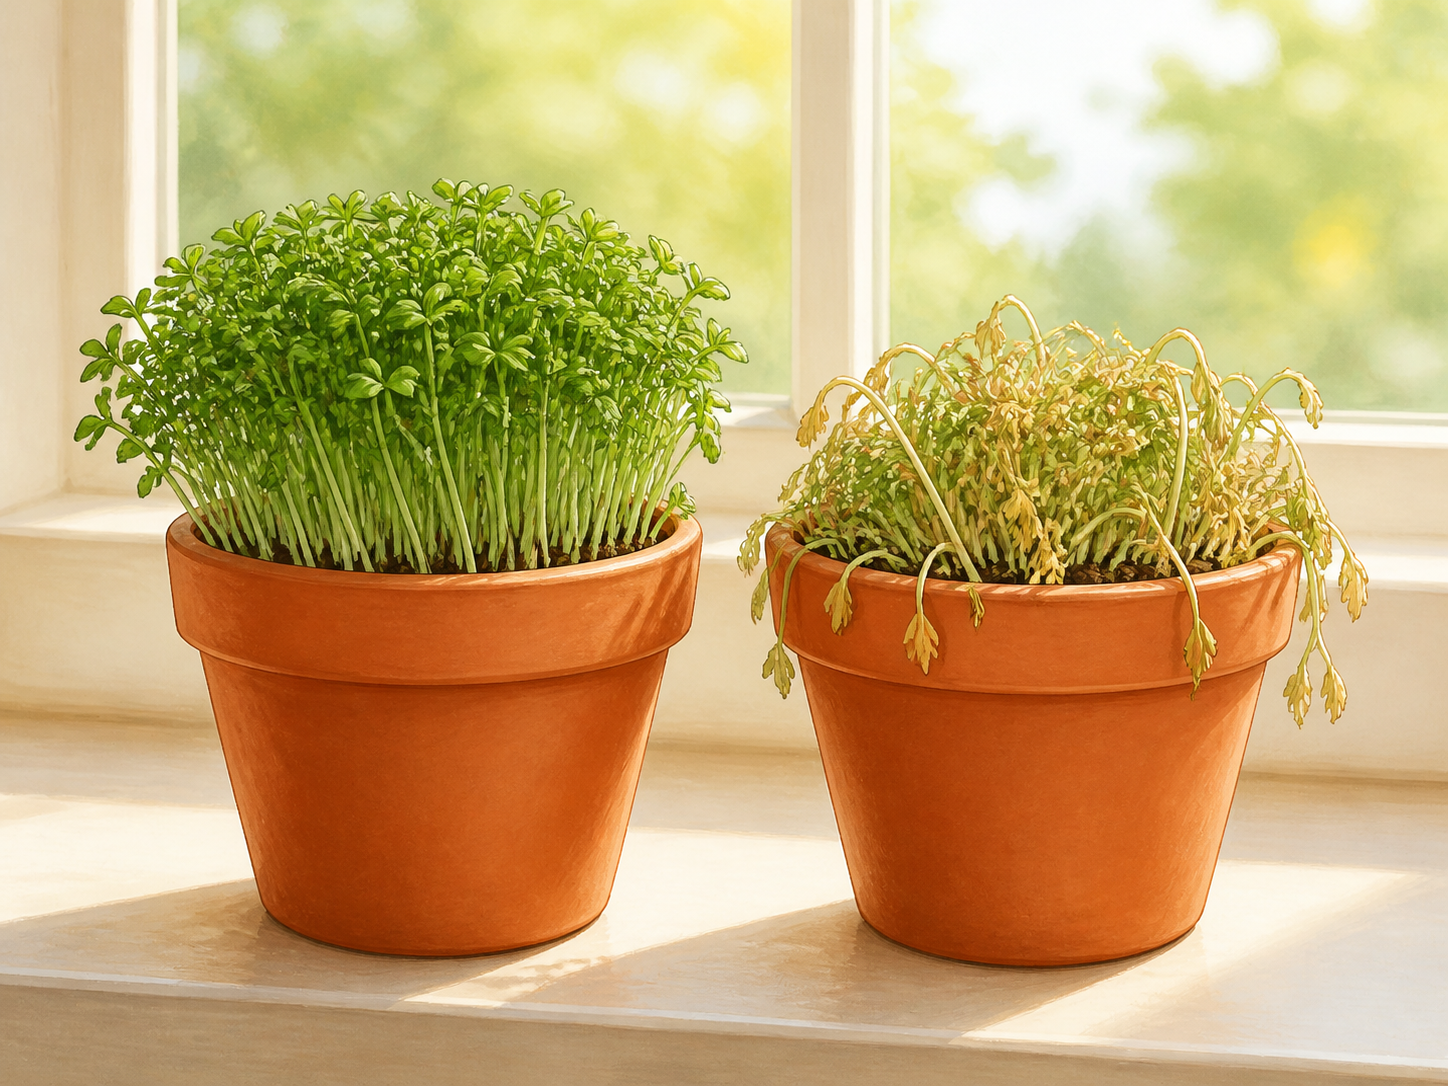
\includegraphics[width=0.58\linewidth]{images/book1/ai/g4-plants-cresspots.png}

{\small El mismo experimento en un alféizar de verdad, una semana
después: las gemelas se diferencian ya en todo lo que se ve ---
porque se diferenciaban en una sola cosa.}
\end{omfigure}

\section{Lo que revelan las pruebas}

\begin{proposition}[Las necesidades de una planta]\label{prop:g4:what-plants-need:needs}
Las pruebas justas, hechas para cada necesidad por turno, enseñan que
una \omterm{def:g1:plants-around-us:plant}{planta} necesita:
\begin{itemize}
  \item \emph{agua} --- la maceta sin regar se marchita y muere;
  \item \emph{luz} --- la maceta del armario crece pálida, larga y
        débil, y después se rinde: sin luz no se fabrica alimento;
  \item \emph{aire} --- encerrada lejos del aire fresco, deja de
        crecer;
  \item \emph{calor} --- con frío, las \omterm{prop:g3:flowers-fruits-seeds:transform}{semillas} esperan
        (\cref{prop:g2:from-seed-to-plant:needs}) y el crecimiento se
        para en seco;
  \item \emph{sales minerales}\index{sales minerales}: cantidades
        diminutas de sustancias nutritivas que las \omterm{def:g1:plants-around-us:parts}{raíces} beben
        disueltas en el agua de la tierra --- en agua pura sola, una
        \omterm{def:g1:plants-around-us:plant}{planta} se queda corta enseguida.
\end{itemize}
\end{proposition}
\admitted

\begin{example}[El prisionero pálido]\label{ex:g4:what-plants-need:pale}
La prueba del armario del \cref{exo:g1:plants-around-us:8}, hecha como
es debido con una gemela iluminada, da un resultado llamativo: el
prisionero no solo está triste, sino \emph{amarillo pálido} --- ha
dejado de fabricar su sustancia verde --- y raramente \emph{alto},
estirado como si buscara la luz que le falta. Crecer sin luz es gastar
sin ganar; quemadas las reservas de la \omterm{def:g2:from-seed-to-plant:seed}{semilla}, se para.
\end{example}

\begin{remark}[Por qué los hortelanos alimentan la tierra]\label{rem:g4:what-plants-need:soil}
El compost y el estiércol no son ``comidas'' para la \omterm{def:g1:plants-around-us:plant}{planta} --- las
\omterm{def:g1:plants-around-us:plant}{plantas} no se comen a nadie. Reponen las \omterm{prop:g4:what-plants-need:needs}{sales minerales} de la tierra,
que las cosechas se llevan año tras año. El cubo de compost del
\cref{ex:g2:caring-for-nature:compost} cierra el círculo: lo que la
tierra les dio a las verduras, las peladuras se lo devuelven a la
tierra.
\end{remark}

\section{Qué hacen las plantas con lo que toman}

\begin{proposition}[Las plantas fabrican su propia materia]\label{prop:g4:what-plants-need:make}
Los \omterm{def:g1:animals-around-us:animal}{animales} crecen comiéndose a otros \omterm{def:g1:living-or-not:living}{seres vivos}. Una \omterm{def:g1:plants-around-us:plant}{planta} no se
come a nadie: con el agua y las \omterm{prop:g4:what-plants-need:needs}{sales minerales} de la tierra, el aire
y la \omterm{prop:g3:balanced-diet:jobs}{energía} de la \emph{luz} que atrapan sus \omterm{def:g1:plants-around-us:parts}{hojas} verdes,
\emph{fabrica su propia materia} --- \omterm{def:g1:plants-around-us:parts}{tallos}, \omterm{def:g1:plants-around-us:parts}{hojas}, \omterm{def:g1:plants-around-us:parts}{raíces} y \omterm{prop:g3:flowers-fruits-seeds:transform}{semillas}
nuevos. Por eso la luz es para una \omterm{def:g1:plants-around-us:plant}{planta} un asunto tan serio como la
comida y la bebida, y por eso la \omterm{def:g1:plants-around-us:parts}{hoja} verde mira al cielo.
\end{proposition}
\admitted

\begin{example}[Un árbol casi de la nada]\label{ex:g4:what-plants-need:tree}
\omterm{def:g1:plants-around-us:plant}{Planta} una pepita en una maceta grande con la tierra pesada, espera
años y allí habrá un arbolito --- y sin embargo la tierra casi no ha
perdido peso. La madera del árbol no salió de la maceta a cucharadas:
se \emph{fabricó}, a partir de agua, aire y luz, en los talleres
verdes de las \omterm{def:g1:plants-around-us:parts}{hojas}. De dónde sale la materia de los \omterm{def:g1:living-or-not:living}{seres vivos} nos
volverá a ocupar en cursos posteriores.
\end{example}

\begin{remark}[El verde le da de comer a todo el mundo]\label{rem:g4:what-plants-need:everyone}
Acuérdate de la \cref{prop:g3:food-chains:start}: toda \omterm{def:g3:food-chains:chain}{cadena
alimentaria} empieza por una \omterm{def:g1:plants-around-us:plant}{planta}. Ahora vemos por qué tiene que ser
así --- las \omterm{def:g1:plants-around-us:plant}{plantas} son el único eslabón que fabrica materia nueva a
partir de ingredientes no vivos. Todos los bocados que come cualquiera,
en cualquier sitio, se fabricaron antes en una \omterm{def:g1:plants-around-us:parts}{hoja}.
\end{remark}

\section{Ejercicios}

\begin{exercise}[$\star$]\label{exo:g4:what-plants-need:1}
Enumera las cinco necesidades de una \omterm{def:g1:plants-around-us:plant}{planta}.
\end{exercise}

\begin{exercise}[$\star$]\label{exo:g4:what-plants-need:2}
En una prueba justa, ¿cuántas cosas pueden ser distintas entre las dos
macetas? ¿Cómo se llama la maceta que no se toca?
\end{exercise}

\begin{exercise}[$\star$]\label{exo:g4:what-plants-need:3}
Describe el aspecto de una \omterm{def:g1:plants-around-us:plant}{planta} que ha pasado quince días a oscuras.
¿Qué necesidad le faltaba y qué no pudo fabricar?
\end{exercise}

\begin{exercise}[$\star$]\label{exo:g4:what-plants-need:4}
¿Qué son las \omterm{prop:g4:what-plants-need:needs}{sales minerales} y cómo las toma la \omterm{def:g1:plants-around-us:plant}{planta}?
\end{exercise}

\begin{exercise}[$\star$]\label{exo:g4:what-plants-need:5}
¿Por qué esparcen compost los hortelanos, si las \omterm{def:g1:plants-around-us:plant}{plantas} no comen?
\end{exercise}

\begin{exercise}[$\star$]\label{exo:g4:what-plants-need:6}
¿En qué se diferencia la manera de crecer de una \omterm{def:g1:plants-around-us:plant}{planta} de la de un
\omterm{def:g1:animals-around-us:animal}{animal}, según la \cref{prop:g4:what-plants-need:make}?
\end{exercise}

\begin{exercise}[$\star$]\label{exo:g4:what-plants-need:7}
En el \cref{ex:g4:what-plants-need:tree}, la tierra de la maceta casi
no perdió peso mientras el árbol crecía. ¿De dónde salió la materia
del árbol?
\end{exercise}

\begin{exercise}[$\star$]\label{exo:g4:what-plants-need:8}
Pruébalo: diseña y haz con berros la prueba justa del agua de la
figura --- dos macetas, una diferencia. Anota lo que veas al cabo de
una semana.
\end{exercise}

\begin{exercise}[$\star\star$]\label{exo:g4:what-plants-need:9}
Lucas ``demuestra'' que las \omterm{def:g1:plants-around-us:plant}{plantas} necesitan música: le cantó a una
maceta durante un mes y creció estupendamente. ¿Qué le falta a su
experimento, según el \cref{met:g4:what-plants-need:fairtest}? Diseña
la versión que lo probaría de verdad.
\end{exercise}

\begin{exercise}[$\star\star$]\label{exo:g4:what-plants-need:10}
Una \omterm{def:g1:plants-around-us:plant}{planta} acuática crece completamente sumergida y sin \omterm{def:g1:plants-around-us:parts}{raíces}, y aun
así está sana. ¿Qué necesidad de las cinco está cubriendo claramente y
cómo --- y qué necesidad le aporta su agua en lugar de la tierra?
\end{exercise}

\begin{exercise}[$\star\star\star$]\label{exo:g4:what-plants-need:11}
Dos macetas idénticas de menta: una en arena con agua de lluvia pura y
otra en tierra de jardín, las dos regadas e iluminadas igual. A los
dos meses la maceta de arena está pequeña y amarilleando. ¿Qué
necesidad aísla esta prueba justa --- y por qué creció al principio la
\omterm{def:g1:plants-around-us:plant}{planta} de la arena?
\end{exercise}
